% ICASSP-ready anonymous draft. Compile from paper/ with IEEEtran available.
\documentclass[conference]{IEEEtran}
\usepackage{graphicx}
\usepackage{amsmath}
\usepackage{booktabs}
\graphicspath{{figures/}}

\title{Decision-Critical Replica Repair for Lossy Multi-Robot Map Sharing}
\author{Anonymous Authors}

\begin{document}
\maketitle

\begin{abstract}
Sparse remote map updates can be lost precisely when a robot must choose a
route. We formulate this as \emph{decision-critical replica inconsistency} and
introduce Path-Scoped Utility-Triggered Replica Repair (PSR-UT): a versioned
anti-entropy protocol that queries only an imminent planning corridor and only
when optimistic and pessimistic local A* plans disagree on the next action. In
a 100-map matched comparison under 30\% loss, PSR-UT raises completion
success from 0.8400 to 0.9325 versus one-shot sharing for 10.4~KB extra
attempted traffic per episode. Periodic full anti-entropy reaches 0.9575 but
uses 3.8$\times$ the traffic; reliable ARQ is more successful (0.9762) at a
similarly higher traffic point. Ablations identify both the utility trigger and
repair deadline, while independent topologies, densities, delays, and scales
bound the claim to time-critical route decisions.
\end{abstract}

\begin{IEEEkeywords}
multi-robot systems, map sharing, lossy communication, replicated state,
multi-agent path finding
\end{IEEEkeywords}

\section{Introduction}
Robots with local sensing often exchange map state. A dropped cell update can
leave one receiver with a stale replica; if the cell lies on an imminent route,
the receiver may commit before local sensing resolves the uncertainty. This is
not a general claim that every replica mismatch matters. Rather, it is a
specific failure mode of one-shot explicit map sharing under a decision
deadline.

We study an explicit-state systems question instead of replacing the planner or
learning a latent communication policy. Existing learned communication systems
optimize different representations and coordination objectives
\cite{ma2021dcc,wang2023scrimp}. Here every policy uses the same fixed A*, cell
delta representation, topology, instance, and lossy trace; only missing-state
recovery changes. The resulting contribution is a controlled reliability--
traffic operating point for decision-critical replica repair.

PSR-UT has two receiver-local gates. A spatial gate limits repair to an
imminent path corridor. A utility gate sends the stamped digest only when an
optimistic map and a pessimistic interpretation of unknown cells imply
different next actions. Its contributions are: (i) a concrete formulation of
decision-critical replica inconsistency, (ii) a two-gate, truth-map-free repair
protocol, and (iii) matched ablation and extension evidence that reports both
its operating point and its delay/scale boundaries.

\section{Replica Repair Protocol}
Each robot maintains a versioned cell map $M_i^t$. A cell carries a
lexicographically ordered stamp containing version, observation time, sender,
and state tie break. An incoming cell is merged only if its stamp dominates the
local stamp. Normal observations are directed one-shot deltas. Data, digest,
acknowledgement, and repair bytes all traverse the same directed lossy channel.

We use an executable fixed-width wire format rather than object-level traffic
estimates. A cell delta is 13 bytes, including provenance, coordinates, state,
version, observation time, and CRC16. A query over $n$ stamped cells is
$16+6n$ bytes, a patch returning $m$ cells is $4+13m$ bytes, an ACK is 8 bytes,
and a replica digest is 16 bytes. The six-byte query entry bit-packs bounded
coordinates and the complete requester stamp. Update identifiers are
deterministically reconstructed and are not transmitted. The channel carries
the resulting byte strings; decoders reject invalid lengths, versions, bounds,
reserved bits, or checksums before applying the same dominating-stamp merge.
All attempted encoded bytes, including lost packets, count as traffic.

For receiver $j$, fixed A* produces path $\pi_j^t$. Its candidate repair region
is the dilated imminent corridor
\begin{equation}
\mathcal{R}_j^t = \operatorname{Dilate}(\pi_j^t[1:H], r),
\end{equation}
where $H$ is the look-ahead horizon and $r$ the Manhattan radius. A receiver
queries a peer with only the cells and stamps in $\mathcal{R}_j^t$; the peer
returns only dominating cells. PSR-UT then applies a local utility test:
\begin{equation}
a_j^{\mathrm{opt}} \neq a_j^{\mathrm{pess}}.
\end{equation}
The operational map yields $a_j^{\mathrm{opt}}$ and treating unknown corridor
cells as blocked yields $a_j^{\mathrm{pess}}$. A query is suppressed when they
agree. Thus the corridor specifies \emph{where} a repair can matter and action
disagreement specifies \emph{when} it is decision-critical; neither computation
uses the ground-truth map or a learned predictor.

\begin{figure}[t]
  \centering
  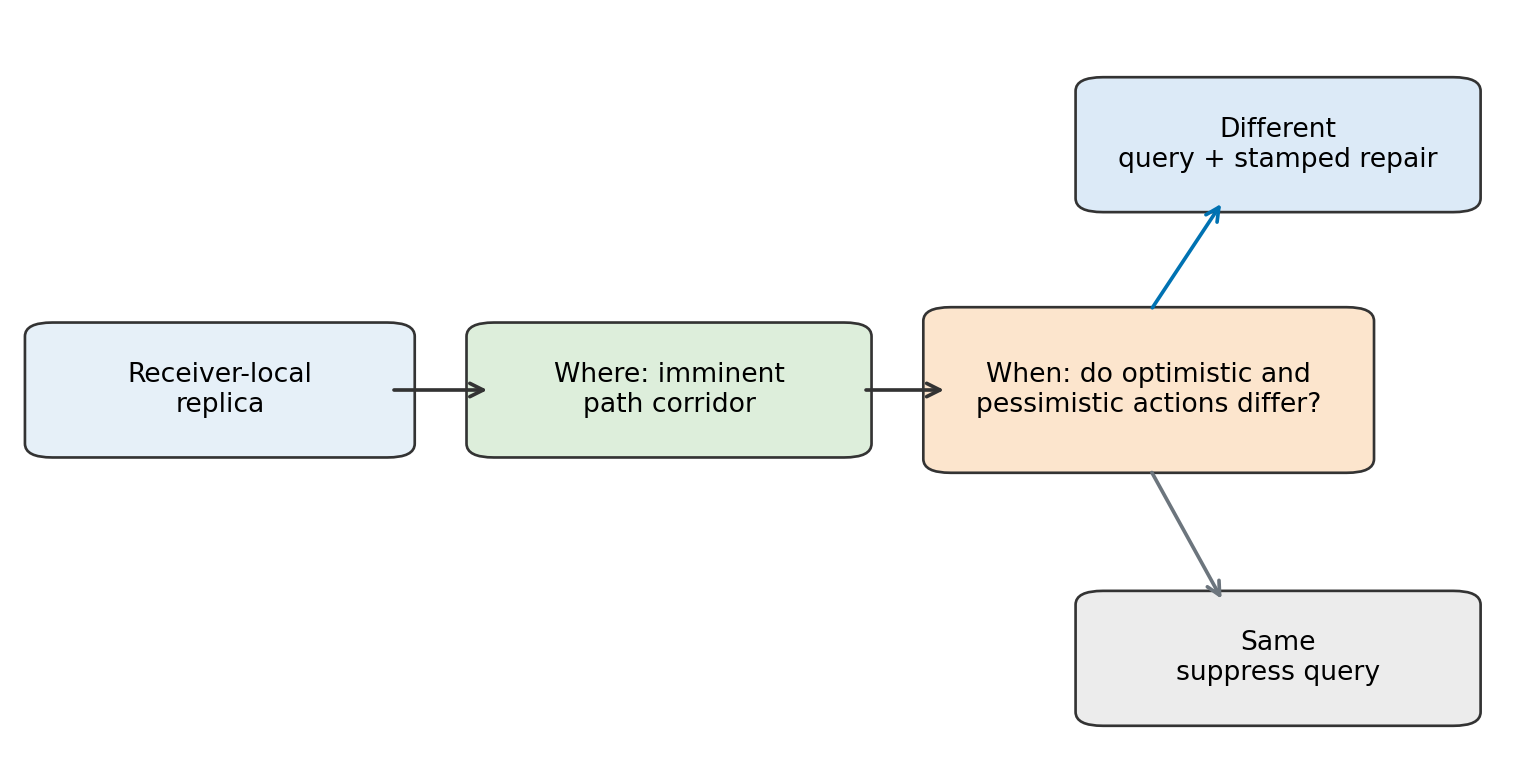
\includegraphics[width=\columnwidth]{psr_ut_two_gate_schematic.png}
  \caption{PSR-UT first restricts repair to the imminent path corridor, then
  issues a digest only if local optimistic and pessimistic actions differ.}
  \label{fig:two-gate}
\end{figure}

\section{Experimental Protocol}
The primary task is an eight-robot shared-map decision geometry: remote
observers can see a blocked branch before paired seekers reach a fork, while
seekers cannot locally observe the branch before committing. Every comparison
uses 100 independent maps, each paired across policies with one independent
loss trace, fixed A*, and identical per-step budgets. We report trial-level
means, sample standard deviations, and a 20,000-draw bootstrap over maps.

Primary controls are One-shot Unique Delta, Retry-All ARQ, Path-Weighted ARQ,
Periodic Full Anti-Entropy (K=4), Mismatch-Triggered Full Replica Repair, and
PSR-UT. The ablations change one
factor: utility trigger versus an action-triggered repair control, cadence 1
versus 4, and corridor repair versus full-replica repair. Extensions sweep
loss, obstacle density, link delay, agent/map scale, and three independent
decision geometries. Random-map conditions are retained as negative controls.

\section{Results}
At 30\% loss, PSR-UT improves One-shot completion success by $+0.0925$
(paired 95\% CI $[+0.0750,+0.1100]$) for 10,422 additional attempted bytes.
It does not claim universal dominance: Periodic Full (K=4) attains 0.9575
success but needs 285.8~KB per episode, while Retry-All and Path-Weighted ARQ
reach about 0.98 with approximately 264~KB, versus 75.8~KB for PSR-UT.
Mismatch-triggered full repair is both less reliable and much more expensive.
The primary confidence intervals bootstrap independent maps.

\begin{table}[t]
\caption{Primary comparison at 30\% loss: 100 independent maps, bootstrap 95\% CIs.}
\label{tab:primary}
\centering
\small
\begin{tabular}{lcc}
\toprule
Method & CSR & Attempted KB \\
\midrule
One-shot & .8400 [.8200,.8600] & 65.4 [65.1,65.6] \\
PSR-UT & .9325 [.9163,.9475] & 75.8 [75.5,76.0] \\
Retry-All ARQ & .9762 [.9650,.9862] & 263.9 [263.1,264.7] \\
Path-Weighted ARQ & .9775 [.9663,.9875] & 263.9 [263.1,264.7] \\
Periodic Full (K=4) & .9575 [.9437,.9700] & 285.8 [282.7,289.0] \\
Mismatch Full & .9150 [.8975,.9313] & 578.9 [572.6,585.0] \\
\bottomrule
\end{tabular}
\end{table}

\begin{figure}[t]
  \centering
  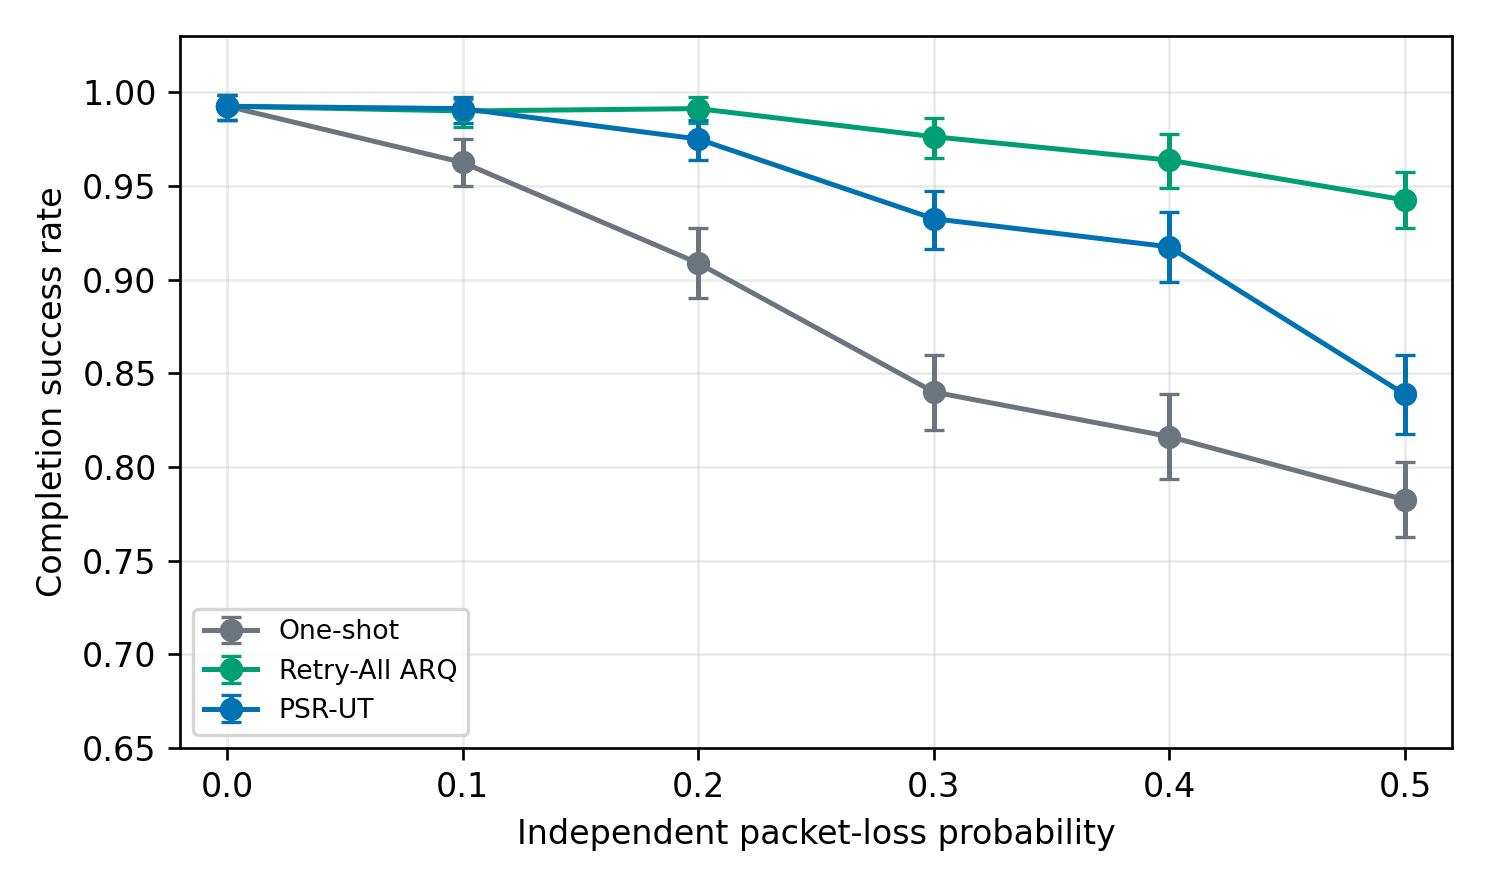
\includegraphics[width=\columnwidth]{psr_ut_csr_vs_loss.png}
  \caption{Loss sweep. PSR-UT improves on One-shot over the tested nonzero
  loss range while occupying a lower-traffic point than ARQ.}
  \label{fig:loss}
\end{figure}

\begin{figure}[t]
  \centering
  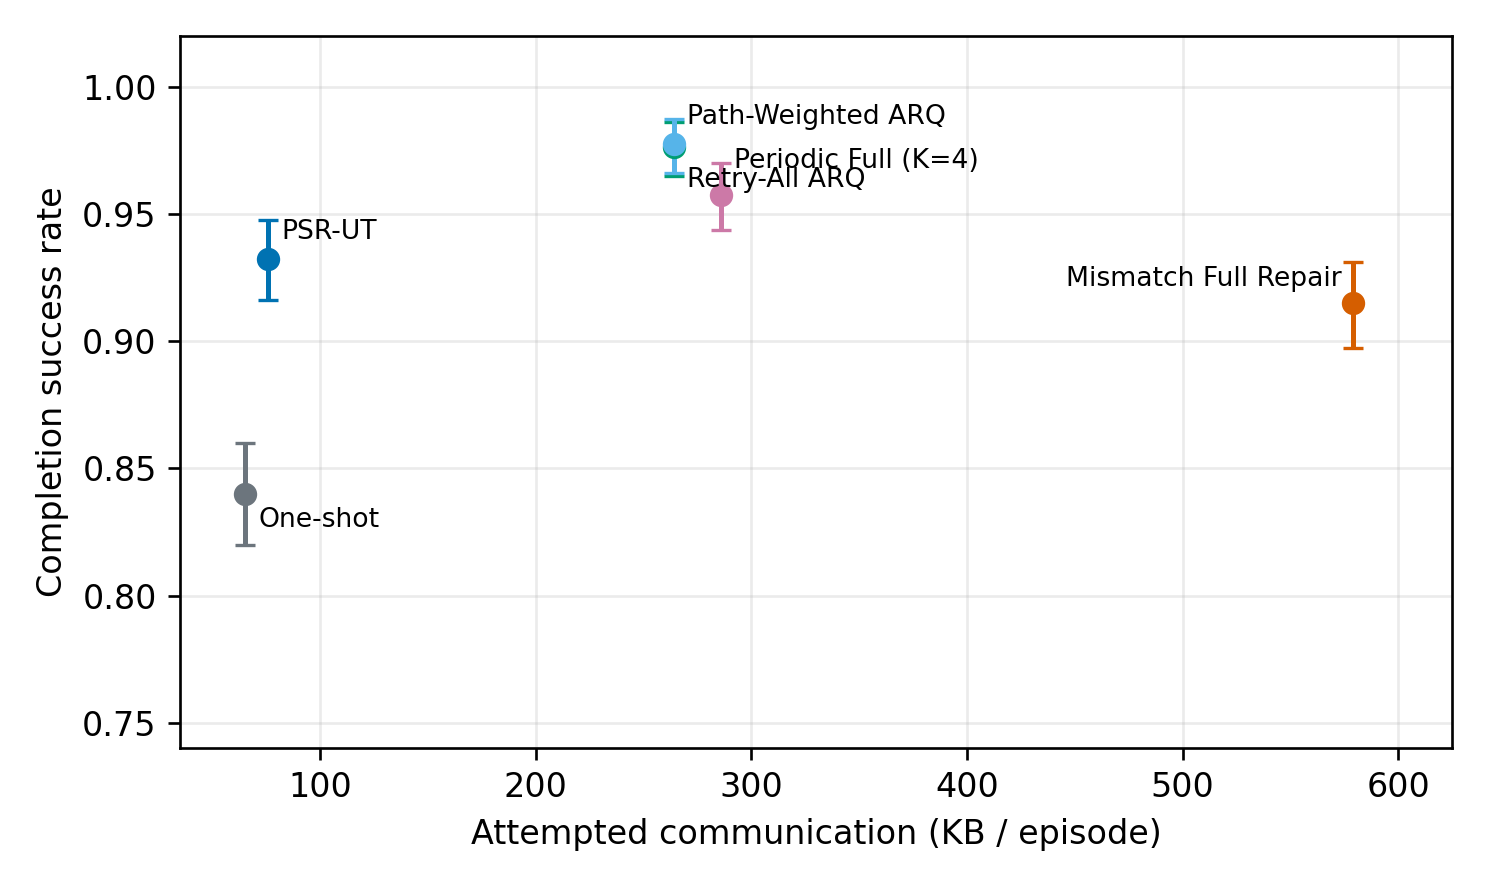
\includegraphics[width=\columnwidth]{psr_ut_primary_pareto.png}
  \caption{The primary reliability--traffic frontier. PSR-UT is an
  intermediate operating point, not a replacement for unconstrained ARQ.}
  \label{fig:pareto}
\end{figure}

The ablations support the two gates. Replacing PSR-UT with action-triggered
repair reduces CSR from 0.9325 to 0.8400 ($+0.0925$ for PSR-UT,
$[+0.0750,+0.1100]$). Changing only the repair cadence from every step to
every four steps reduces CSR to 0.8488, exposing the decision deadline.
Changing only the repair scope to a full replica reduces CSR to 0.8400 and
increases traffic from 75.8 to 174.0~KB; paired changes are $+0.0925$ CSR and
$-98.2$~KB in favor of PSR-UT.

The extensions delimit the result. PSR-UT achieves CSR 0.9913, 0.9750,
0.9325, 0.9175, and 0.8388 at loss probabilities 0.1 through 0.5. At one,
two, and four delivery steps, CSR decreases to 0.9075, 0.8550, and 0.7388,
respectively. Across 4/8/16/32 agents, its paired improvement over One-shot
is positive but small: $+0.0050$ to $+0.0003$. It improves over One-shot in
T-junction, asymmetric-fork, and narrow-bypass validations by $+0.1163$,
$+0.1175$, and $+0.1275$ CSR. In random-map negative controls, PSR-UT and
One-shot are approximately equivalent. These controls show that replica repair
matters when a missing update changes an imminent route, not for arbitrary map
disagreement.

\section{Conclusion}
PSR-UT repairs explicit map replicas only when state lies near an imminent
route and local uncertainty can change the next action. Under loss it improves
upon one-shot sharing with modest added traffic, while reliable ARQ remains the
higher-traffic reliability endpoint. Matched ablations, scales, topologies, and
negative controls make the appropriate claim specific: decision-critical
replica repair before a communication deadline.

\bibliographystyle{IEEEtran}
\bibliography{psr_icassp_refs}
\end{document}
